\section{Introdução}

\begin{frame}

    \frametitle{Motivação}

    \begin{columns}[c]

        \begin{column}{0.48\textwidth}
            \begin{itemize}
                \item Robôs reais sofrem com \alert{ruído de sensores} e \alert{perturbações} (ex.: vento).
                \item O robô só tem uma \textbf{crença} sobre o estado: $\boldsymbol{\mu}$ e $\boldsymbol{\Sigma}$ de um EKF.
                \item Controladores de segurança clássicos usam só a média e \alert{descartam a incerteza}.
            \end{itemize}

            \begin{block}{Objetivo}
                ``A probabilidade de sair da região segura deve ser menor que 1\%.''
            \end{block}
        \end{column}

        \begin{column}{0.48\textwidth}
            \centering
            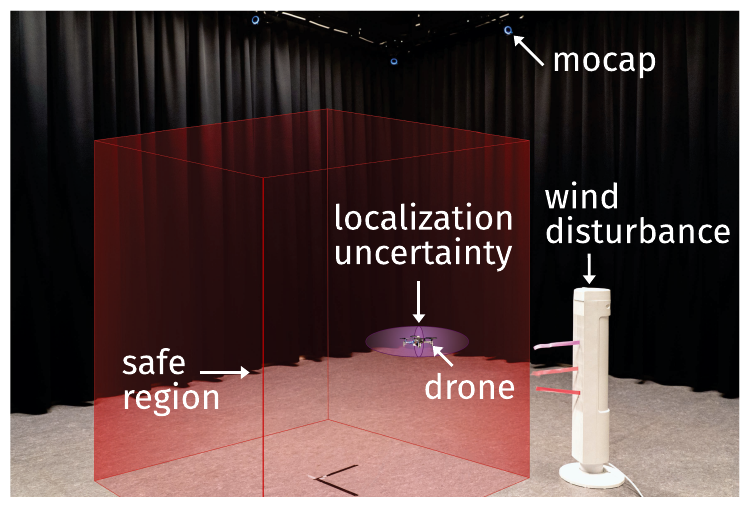
\includegraphics[width=\textwidth]{imagens/fig1_quadrotor}

            {\tiny Fonte: \citeonline{vahs2023bcbf}.}
        \end{column}

    \end{columns}

\end{frame}
